\chapter{Modelo para conformar equipos de béisbol y docentes basado en TEAMSOFT$^+$}\label{chap:2}

En el presente capítulo se describe cómo pueden definirse los problema de conformación de equipos de béisbol y docentes empleando como base el modelo para la formación de equipos de proyectos de software soportado por la herramienta \hyperref[sec:modelo-teamsoft]{TEAMSOFT$^+.$} Esto implica que para cada problema se utilizarán o no, algunas de las relaciones propuestas en este modelo. También se describe una propuesta para obtener los valores de las competencias de las personas a partir de información que hoy se gestiona sobre ellas.

\section{Ejemplo simple para el problema de conformación de equipos de béisbol}\label{ejemplo-pel}

Partiendo del modelo de conformación de equipos de software, descrito en la sección \ref{sec:modelo-teamsoft}, se ejemplificará con una instancia, una aproximación del problema de conformación de equipos de béisbol. Se recomienda el análisis futuro de otros roles como el emergente o los roles asociados al picheo como abridores o relevistas que tienen otra complejidad.

\subsection{Conjuntos que intervienen en la modelación}\label{sec:conjuntos}
Un equipo está compuesto por una nómina de jugadores, generalmente más de 20, entre los cuales se escoge la alineación regular. Esta alineación se compone de 10 jugadores que tienen que jugar 18 roles. Estos roles están divididos en dos categorías o tipos (ver Tabla \ref{tipo-roles}).

\begin{table}[H]
	\centering
	\caption{Tipos de Roles}\label{tipo-roles}
	\scalebox{0.95}{
	\begin{tabular}{l	 c}
		\toprule[1.7pt]
		\textbf{Roles defensivos} & \textbf{Roles Ofensivos} \\ \midrule
		      receptor (C)        & 1$^{er}$ bate (B1)       \\
		      1ra base (1B)       & 2$^{do}$ bate (B2)       \\
		      2da base (2B)       & 3$^{er}$ bate (B3)       \\
		    campo corto (SS)      & 4$^{to}$ bate (B4)       \\
		      3ra base (3B)       & 5$^{to}$ bate (B5)       \\
		jardinero izquierdo (LF)  & 6$^{to}$ bate (B6)       \\
		 jardinero central (CF)   & 7$^{mo}$ bate (B7)       \\
		 jardinero derecho (RF)   & 8$^{vo}$ bate (B9)       \\
		 bateador designado (BD)  & 9$^{no}$ bate (B9)       \\ \bottomrule[1pt]
	\end{tabular}
}
\end{table}

\begin{itemize}	
	\item $P=\{p_1, p_2\ldots\}$: Conjunto de jugadores, $p = 1...|25|$.
	
	\item $T=\{t_1=batear\;con\;hombres\;en\;base, t_2=fuerza\;de\;bateo, t_3=precisi\acute{o}n\;de\;tiro, t_4=velocidad, t_5=versatilidad, t_6=capacidad\;de\;embase\}$: Conjunto de competencias técnicas, $t= 1\ldots|T|$, $|T|=6$. \label{compt-pel}
	
	\item $G=\{g_1=trabajo\;bajo\;presi\acute{o}n
	, g_2=libre\;de\;preocupaciones, g_3=concentraci\acute{o}n,$ $g_4=afrontar\;la\;adversidad, g_5=preparaci\acute{o}n\;mental, g_6=entrenabilidad,$ $g_7=motivaci\acute{o}n\;para\;el\;logro\}$: Conjunto de competencias genéricas, $g= 1\ldots |G|$, $|G|=7$.
	
	\item $R=\{r_1=C,r_2=1B,r_3=2B,r_4=SS,r_5=3B,r_6=LF,r_7=CF,r_8=RF,r_{9}=BD,r_{10}=B1,r_{11}=B2,r_{12}=B3,r_{13}=B4,r_{14}=B5,r_{15}=B6, r_{16}=B7,r_{17}=B8,r_{18}=B9\}$: Conjunto de roles, $r = 1\ldots |R|$, $|R|=18$. \label{def-roles-pel} 
	
	\item $Y={y_1}$: Un solo equipo a conformar.
	
\end{itemize}


Las relaciones se van a dividir en dos secciones. La primera sección trata los aspectos genéricos del problema, que no cambian en función de los integrantes, o del equipo. La segunda sección va a un nivel más específico, que está en dependencia de las personas a asignar. Los valores asignados en la sección \ref{asp-gen-pel} son todos a consideración del autor, y además, son configurables.

\subsection{Elementos generales} \label{asp-gen-pel}

En las Tablas \ref{mcgd-pel} y \ref{mcgo-pel} se muestran los valores mínimos necesarios que las personas deben tener en las competencias genéricas para desempeñar cada rol. Por ejemplo, para poder jugar el rol $C$ es necesario que la persona tenga como mínimo un valor en la competencia genérica $g_1$ de 0.8. 

 
\begin{table}[H]
	\caption{Valores mínimos de las competencias genéricas para cada rol defensivo}\label{mcgd-pel}
	\centering
	\begin{tabular}{|l|c|c|c|c|c|c|c|c|c|}
		\hline
		$Z(g,r)$ & $C$ & $1B$  & $2B$ & $SS$ & $3B$ & $LF$ & $CF$ & $RF$ & $BD$ \\ \hline
		$g_1=trabajo\;bajo\;presi\acute{o}n$ & 0.8 & 0.6 & 0.6 & 0.6 & 0.6 & 0.5 & 0.5 & 0.5 & 0.3
		\\ \hline
		$g_2=libre\;de\;preocupaciones$ & 0.7 & 0.6 & 0.7 & 0.7 & 0.6 & 0.7 & 0.7 & 0.7 & 0.3\\ \hline
		$g_3=concentraci\acute{o}n$ & 0.8 & 0.7 & 0.7 & 0.7 & 0.7 & 0.6 & 0.6 & 0.6 & 0.5 \\ \hline
		$g_4=afrontar\;la\;adversidad$ & 0.6 & 0.5 & 0.5 & 0.5 & 0.5 & 0.5 & 0.4 & 0.4 & 0.3 \\ \hline
		$g_5=preparaci\acute{o}n\;mental$ & 0.7 & 0.3 & 0.3 & 0.3 & 0.3 & 0.3 & 0.3 & 0.3 & 0.3 \\ \hline
		$g_6=entrenabilidad$ & 0.5 & 0.5 & 0.5 & 0.5 & 0.5 & 0.5 & 0.5 & 0.5 & 0.4\\ \hline
		$g_7=motivaci\acute{o}n\;para\;el\;logro$ & 0.5 & 0.5 & 0.5 & 0.5 & 0.5 & 0.5 & 0.5 & 0.5 & 0.4\\ \hline
	\end{tabular}
\end{table}

\begin{table}[H]
	\caption{Valores mínimos de las competencias genéricas para cada rol ofensivo}\label{mcgo-pel}
	\centering
	\begin{tabular}{|l|c|c|c|c|c|c|c|c|c|}
		\hline
		\thead{$Z(g,r)$} & $B1$ & $B2$  & $B3$ & $B4$ & $B5$ & $B6$ & $B7$ & $B8$ & $B9$ \\ \hline
		$g_1=trabajo\;bajo\;presi\acute{o}n$ 	 & 0.6 	&  0.6 	&  0.7 &  0.7 &  0.7 &  0.5 &  0.5 & 0.5  & 0.4 \\ \hline
		$g_2=libre\;de\;preocupaciones$ 	 & 0.5  &  0.5  &  0.5 &  0.5 &  0.4 &  0.4 &  0.4 & 0.4  & 0.3 \\ \hline
		$g_3=concentraci\acute{o}n$ 	 & 0.7  &  0.7  &  0.7 &  0.7 &  0.7 &  0.6 &  0.6 & 0.6  & 0.5 \\ \hline
		$g_4=afrontar\;la\;adversidad$ 	 & 0.6  &  0.5  &  0.5 &  0.5 &  0.5 &  0.5 &  0.4 & 0.4  & 0.3 \\ \hline
		$g_5=preparaci\acute{o}n\;mental$ 	 & 0.7  &  0.6  &  0.6 &  0.7 &  0.7 &  0.6 &  0.5 & 0.5  & 0.4 \\ \hline
		$g_6=entrenabilidad$ 	 & 0.5  &  0.5  &  0.5 &  0.5 &  0.5 &  0.5 &  0.5 & 0.5  & 0.5 \\ \hline
		$g_7=motivaci\acute{o}n\;para\;el\;logro$ 	 & 0.6  &  0.6  &  0.6 &  0.6 &  0.6 &  0.6 &  0.6 & 0.6  & 0.6 \\ \hline
	\end{tabular}
\end{table}


%--------inicio-y1-------------
 
En las Tablas \ref{mctd1-pel} y \ref{mcto1-pel} se muestran los valores mínimos necesarios que las personas deben tener en las competencias técnicas para desempeñar cada rol. Las posiciones defensivas no requieren de competencias relacionadas con la ofensiva ($t_1=$ \textit{batear con hombres en base} y $t_2=$ \textit{fuerza de bateo}), por lo tanto, a cada rol defensivo se le otorga el valor de 0.0 en las competencias relacionadas con la ofensiva. El bateador designado es un caso excepcional, aunque clasificado como un rol defensivo, no tiene competencias defensivas que lo definan como tal. Esto significa que, aunque realmente no juega a la defensiva, es necesario tenerlo en cuenta para ocupar un rol a la ofensiva. Por lo tanto, se asocian a este rol, las competencias que tienen tendencia ofensiva.
\begin{table}[H]
	\caption{Valores mínimos de las competencias técnicas para cada rol defensivo en el equipo $y_1$}\label{mctd1-pel}
	\begin{tabular}{|l|c|c|c|c|c|c|c|c|c|}
		\hline
		\thead{$Q(t,r,y)$} & $C$ & $1B$  & $2B$ & $SS$ & $3B$ & $LF$ & $CF$ & $RF$ & $BD$  \\ \hline
		$t_3=precisi\acute{o}n\;de\;tiro$ 		 & 0.8 &  0.5  &  0.6 & 0.6  & 0.7  & 0.7  & 0.7  &  0.7 & 0.0 \\ \hline
		$t_4=velocidad$ 		 & 0.2 &  0.2  &  0.2 & 0.2  & 0.2  & 0.7  & 0.8  &  0.7 &  0.4 \\ \hline
		$t_5=versatilidad$   	 & 0.2 &  0.3  &  0.5 & 0.5  & 0.5  & 0.6  & 0.6  &  0.6 & 0.0 \\ \hline
		$t_6=capacidad\;de\;embase$ & 0.2 &  0.2  &  0.2 & 0.2  & 0.0  & 0.3  & 0.3  &  0.6 & 0.6 \\ \hline
	\end{tabular}
\end{table}

Los roles ofensivos no necesitan tener habilidades defensivas, como es el caso de la competencia técnica $t_3=precisi\acute{o}n\;de\;tiro$. Por este motivo no se muestra en la Tabla \ref{mcto1-pel}.

\begin{table}[H]
	\centering
	\caption{Valores mínimos de las competencias técnicas para cada rol ofensivo en el equipo $y_1$}\label{mcto1-pel}
	\begin{tabular}{|l|c|c|c|c|c|c|c|c|c|}
		\hline
		\thead{$Q(t,r,y)$} & $B1$ & $B2$ & $B3$ & $B4$ & $B5$ & $B6$ & $B7$ & $B8$ & $B9$  \\ \hline
		$t_1=batear\;con\;hombres\;en\;base$ 	     & 0.6  & 0.7  & 0.8  & 0.8  & 0.7  & 0.7  & 0.5  & 0.5  & 0.5 \\ \hline
		$t_2=fuerza\;de\;bateo$ 		 & 0.5  & 0.6  & 0.7  & 0.8  & 0.7  & 0.6  & 0.5  & 0.4  & 0.4 \\ \hline
		$t_4=velocidad$ 		 & 0.7  & 0.5  & 0.4  & 0.3  & 0.3  & 0.3  & 0.3  & 0.2  & 0.1 \\ \hline
		$t_5=versatilidad$   	 & 0.3  & 0.3  & 0.3  & 0.3  & 0.2  & 0.3  & 0.3  & 0.1  & 0.3 \\ \hline
		$t_6=capacidad\;de\;embase$ & 0.8 &  0.7  &  0.6 & 0.6  & 0.6  & 0.5  & 0.5  &  0.4 & 0.4 \\ \hline
	\end{tabular} 
\end{table}
%----------------fin--y1-----------------


%---------------inicio----------------------

%----------------nuevo----------------

Anteriormente se explicó que en un equipo de pelota, cada jugador ocupa dos roles, uno a la defensiva y otro a la ofensiva. La Tabla \ref{cmrpp-pel} muestra lo planteado.
\begin{table}[H]
	\centering
	\caption{Cantidad máxima de roles por persona a jugar en un equipo de béisbol }\label{cmrpp-pel}
	\begin{tabular}{|c|c|c|c|c|c|c|c|c|c|}
		\hline
		$K_{py}(p,y)$ & $p_1$ & $p_2$ & $p_3$  & $p_4$ & $p_5$ & $p_6$ & $p_7$  & $p_8$ & $p_9$ \\ \hline
		$y_1$ & 2 & 2 & 2 & 2 & 2 & 2 & 2 & 2 & 2 \\ \hline
	\end{tabular}
\end{table}

%-----------------------------------

Las incompatibilidades entre los roles como ya se mencionaba, está dada por el tipo de rol. Todos los roles ofensivos (por ejemplo, B1, B2, B3) tienen incompatibilidades entre ellos, y son compatibles con los defensivos (por ejemplo, C, 3B, CF). Los roles defensivos, al igual que los ofensivos, son incompatibles entre ellos, siendo compatibles además con los defensivos. Por cuestión de una mejor calidad en la visualización de los datos, en la Tabla \ref{ier1-pel} solo se pone un subconjunto de los roles.
\begin{table}[H]
	\centering
	\caption{Incompatibilidades entre roles}\label{ier1-pel}
	\begin{tabular}{|c|c|c|c|c|c|c|}
		\hline
		$I_r(r,u,y)$  & $B1$& $B2$& $B3$& $C$ & $3B$& $CF$  \\ \hline
		$B1$ 			&  0  &  1  &  1  &  0  &  0  &  0 \\ \hline
		$B2$ 			&  1  &  0  &  1  &  0  &  0  &  0 \\ \hline
		$B3$ 			&  1  &  1  &  0  &  0  &  0  &  0 \\ \hline
		$C$		    	&  0  &  0  &  0  &  0  &  1  &  1 \\ \hline
		$3B$			&  0  &  0  &  0  &  1  &  0  &  1 \\ \hline
		$CF$ 			&  0  &  0  &  0  &  1  &  1  &  0 \\ \hline
	\end{tabular}
\end{table}


La cantidad de personas necesarias para jugar un rol en una alineación siempre será una sola, sin importar el tipo de rol, y el equipo.\\

\subsection{Elementos específicos} \label{asp-espec-pel}

Después de ver los aspectos generales del modelo, es necesario instanciar tanto las personas como el equipo en cuestión, para lograr un ejemplo completo. Todos los valores otorgados en esta sección son ficticios. Más adelante, en la sección \ref{sec:tran_pel} se hace una propuesta para la obtención de estos datos a partir de fuentes externas.

\begin{itemize}
	\item $P=\{p_1=frank, p_2=rudy, p_3=carlos, p_4=alexander, p_5=juan, p_6=yurisbel, p_7=jos\acute{e},p_8=pedro,p_9=pepe, p_{10}=camilo, p_{11}=oscar, p_{12}=roberto, p_{13}=enrique, p_{14}=yasel, p_{15}=dayron\}$: Conjunto de personas, $p = 1...|P|$, $|P|=15$.
	
	\item $Y=Industriales$: Equipo a conformar.
\end{itemize}

En la Tabla \ref{iep-pel} se muestra un ejemplo de las incompatibilidades entre los jugadores del equipo Industriales. Es importante destacar que la relación de incompatibilidad no tiene que ser la misma en ambos sentidos, por ejemplo $p_1$  es totalmente incompatible con $p_2$, mientras que $p_2$ es compatible con $p_1$.

\begin{table}[H]
	\centering
	\caption{Incompatibilidades entre personas del equipo $Industriales$}\label{iep-pel}
	\begin{tabular}{|c|c|c|c|c|c|c|c|c|c|}
		\hline
		$I_p(p,q)$ & $p_1$ & $p_2$ & $p_3$  & $p_4$ & $p_5$ & $p_6$ & $p_7$ & $p_8$  & $p_9$ \\ \hline
		$p_1$ 	& 0.0 & 1.0 & 0.3 & 0.2 & 0.4 & 0.0 & 0.4 & 0.3 & 0.2 \\ \hline
		$p_2$  	& 0.3 & 0.0 & 0.9 & 0.0 & 0.1 & 0.8 & 0.0 & 0.9 & 0.0 \\ \hline
		$p_3$ 	& 0.5 & 0.2 & 0.0 & 0.3 & 0.2 & 0.5 & 0.2 & 0.0 & 0.3 \\ \hline
		$p_4$ 	& 0.6 & 0.3 & 0.5 & 0.0 & 0.3 & 0.3 & 0.5 & 0.0 & 0.3 \\ \hline
		$p_5$ 	& 0.1 & 0.7 & 0.1 & 0.8 & 0.0 & 0.1 & 0.7 & 0.1 & 0.8 \\ \hline
		$p_6$ 	& 0.0 & 1.0 & 0.3 & 0.2 & 0.4 & 0.0 & 0.9 & 0.3 & 0.2 \\ \hline
		$p_7$  	& 1.0 & 0.0 & 0.9 & 0.0 & 0.1 & 1.0 & 0.0 & 0.9 & 0.0 \\ \hline
		$p_8$ 	& 0.5 & 0.2 & 0.0 & 0.3 & 0.2 & 0.5 & 0.2 & 0.0 & 0.3 \\ \hline
		$p_9$ 	& 0.6 & 0.3 & 0.5 & 0.0 & 0.3 & 0.3 & 0.5 & 0.0 & 0.0 \\ \hline
	\end{tabular}
\end{table}


%---------------------inicio--------------

Las personas tienen un valor de preferencia por cada rol. Por ejemplo, en la Tabla \ref{prd-pel} se puede decir que la persona $ p_3 $ tiene poca preferencia por el rol $ 3B $ y un valor de preferencia alto por el rol $ C $.
\begin{table}[H]
	\centering
	\caption{Preferencias de las personas por los roles defensivos}\label{prd-pel}
	\begin{tabular}{|c|c|c|c|c|c|c|c|c|c|}
		\hline
		$F_r(p,r)$ & $C$ & $1B$ & $2B$ & $SS$ & $3B$ & $LF$ & $CF$ & $RF$  & $BD$   \\ \hline
		$p_1$   & 0.6 & 0.2 & 0.5 & 0.6 & 0.8 & 0.6 & 0.2 & 0.5 & 0.6 \\ \hline
		$p_2$   & 0.2 & 0.3 & 0.6 & 0.4 & 0.5 & 0.2 & 0.3 & 0.6 & 0.4 \\ \hline
		$p_3$  	& 0.9 & 0.2 & 0.3 & 0.2 & 0.1 & 0.9 & 0.2 & 0.3 & 0.2 \\ \hline
		$p_4$ 	& 0.7 & 0.1 & 0.1 & 0.3 & 0.2 & 0.7 & 0.1 & 0.1 & 0.3 \\ \hline
		$p_5$   & 0.1 & 1.0 & 0.2 & 0.1 & 0.6 & 0.8 & 1.0 & 0.5 & 0.1 \\ \hline
		$p_6$   & 0.6 & 0.2 & 0.5 & 0.6 & 0.7 & 0.6 & 0.2 & 0.5 & 0.6 \\ \hline
		$p_7$   & 0.2 & 0.3 & 0.6 & 0.4 & 0.5 & 0.2 & 0.3 & 0.6 & 0.4 \\ \hline
		$p_8$  	& 0.9 & 0.2 & 0.3 & 0.2 & 0.1 & 0.9 & 0.2 & 0.3 & 0.2 \\ \hline
		$p_9$ 	& 0.7 & 0.1 & 0.1 & 0.3 & 0.2 & 0.7 & 0.1 & 0.1 & 0.3 \\ \hline
	\end{tabular}
\end{table}

\begin{table}[H]
	\centering
	\caption{Preferencias de las personas por los roles ofensivos}\label{pro-pel}
	\begin{tabular}{|c|c|c|c|c|c|c|c|c|c|}
		\hline
		$F_r(p,r)$ & $B1$& $B2$ & $B3$ & $B4$ & $B5$ & $B6$ & $B7$ & $B8$  & $B9$   \\ \hline
		$p_1$   & 0.7 & 0.3 & 0.6 & 0.4 & 0.5 & 0.6 & 0.1 & 0.7 & 0.5 \\ \hline
		$p_2$   & 0.2 & 0.5 & 0.4 & 0.7 & 0.7 & 0.5 & 0.5 & 0.3 & 0.7 \\ \hline
		$p_3$  	& 0.9 & 0.2 & 0.3 & 0.2 & 0.1 & 0.9 & 0.2 & 0.3 & 0.4 \\ \hline
		$p_4$ 	& 0.7 & 0.1 & 0.1 & 0.3 & 0.2 & 0.7 & 0.1 & 0.1 & 0.3 \\ \hline
		$p_5$   & 0.1 & 1.0 & 0.2 & 0.1 & 0.6 & 0.8 & 1.0 & 0.5 & 0.1 \\ \hline
		$p_6$   & 0.6 & 0.2 & 0.5 & 0.6 & 0.7 & 0.6 & 0.2 & 0.5 & 0.3 \\ \hline
		$p_7$   & 0.9 & 0.3 & 0.6 & 0.4 & 0.5 & 0.2 & 0.3 & 0.6 & 0.4 \\ \hline
		$p_8$  	& 0.5 & 0.6 & 0.4 & 0.7 & 0.5 & 0.3 & 0.7 & 0.8 & 0.3 \\ \hline
		$p_9$ 	& 0.7 & 0.4 & 0.9 & 0.2 & 0.2 & 0.5 & 0.3 & 0.5 & 0.0 \\ \hline
	\end{tabular}
\end{table}

%-----------------------fin-------------------------

En las Tablas \ref{pcg-pel} y \ref{pct-pel} se muestra el nivel que poseen las personas en las competencias genéricas y técnicas. Por ejemplo en la Tabla \ref{pcg-pel}, la persona $ p_1 $ tiene un valor alto en la competencia $ g_1 $.

\begin{table}[H]
	\centering
	\caption{Valor de las personas en las competencias genéricas}\label{pcg-pel}
	\begin{tabular}{|l|c|c|c|c|c|c|c|c|c|}
		\hline
		\thead{$F_g(g,p)$} & $p_1$ & $p_2$ & $p_3$ & $p_4$ & $p_5$ & $p_6$ & $p_7$ & $p_8$ & $p_9$ \\ \hline  
		$g_1=trabajo\;bajo\;presi\acute{o}n$ 	& 0.7 & 0.5 & 0.3 & 0.6 & 0.8 & 0.4 & 0.3 & 0.7 & 0.1 \\ \hline
		$g_2=libre\;de\;preocupaciones$  	& 0.6 & 0.4 & 0.2 & 0.7 & 0.3 & 0.6 & 0.5 & 0.2 & 0.6 \\ \hline
		$g_3=concentraci\acute{o}n$ 	& 0.7 & 0.5 & 0.3 & 0.6 & 0.8 & 0.4 & 0.3 & 0.7 & 0.1 \\ \hline
		$g_4=afrontar\;la\;adversidad$  	& 0.6 & 0.4 & 0.2 & 0.7 & 0.3 & 0.6 & 0.9 & 0.2 & 0.6 \\ \hline
		$g_5=preparaci\acute{o}n\;mental$ 	& 0.7 & 0.5 & 0.3 & 0.6 & 0.8 & 0.9 & 0.3 & 0.7 & 0.1 \\ \hline
		$g_6=entrenabilidad$ 	& 0.5 & 0.6 & 0.4 & 0.3 & 0.5 & 0.7 & 0.5 & 0.6 & 0.2 \\ \hline
		$g_7=motivaci\acute{o}n\;para\;el\;logro$  	& 0.8 & 0.7 & 0.3 & 0.5 & 0.8 & 0.5 & 0.8 & 0.6 & 0.2 \\ \hline
		
	\end{tabular}
\end{table}

\begin{table}[H]
	\centering
	\caption{Valor de las personas en las competencias técnicas}\label{pct-pel}
	\begin{tabular}{|l|c|c|c|c|c|c|c|c|c|}
		\hline
		\thead{$F_g(t,p)$}                   & $p_1$ & $p_2$ & $p_3$ & $p_4$ & $p_5$ & $p_6$ & $p_7$ & $p_8$ & $p_9$ \\ \hline
		$t_1=batear\;con\;hombres\;en\;base$ &  0.6  &  0.7  &  0.8  &  0.7  &  0.5  &  0.9  &  0.6  &  0.7  &  0.8  \\ \hline
		$t_2=fuerza\;de\;bateo$              &  0.7  &  0.8  &  0.6  &  0.7  &  0.1  &  0.5  &  0.2  &  0.3  &  0.3  \\ \hline
		$t_3=precisi\acute{o}n\;de\;tiro$    &  0.5  &  0.3  &  0.4  &  0.2  &  0.6  &  0.7  &  0.3  &  0.8  &  0.8  \\ \hline
		$t_4=velocidad$                      &  0.4  &  0.5  &  0.3  &  0.3  &  0.5  &  0.6  &  0.2  &  0.7  &  0.7  \\ \hline
		$t_5=versatilidad$                   &  0.5  &  0.7  &  0.6  &  0.7  &  0.6  &  0.3  &  0.8  &  0.6  &  0.1  \\ \hline
		$t_6=capacidad\;de\;embase$          &  0.7  &  0.4  &  0.7  &  0.5  &  0.8  &  0.9  &  0.5  &  0.5  &  0.6  \\ \hline
	\end{tabular}
\end{table}

La carga de trabajo empleada en el modelo de TEAMSOFT$^+$ no se utiliza, debido a que los jugadores de pelota no pueden estar en varios equipos de béisbol al mismo tiempo.

%\begin{minipage}{12cm}
%\begin{landscape}

\subsection{Transformación de los datos}\label{sec:tran_pel}

Para llevar a la práctica el modelo descrito en la sección \ref{ejemplo-pel}, es necesario instanciar los conjuntos y relaciones con datos reales del problema. En el caso del problema de béisbol se utilizarán los datos disponibles en el \href{www.beisbolcubano.cu}{sitio web} de la serie nacional cubana (ver Figura \ref{info-pelota}).\\

Mediante la opción de descargas brindada por el portal web, se obtienen estos datos. A continuación se describe brevemente cada indicador agrupado en dos categorías:\\

\large{\textbf{Bateo}:}
\normalsize
\begin{itemize}
	\item \textbf{CB}: comparecencias al bate. Todas las veces que el bateador se dispone a batear.
	\item \textbf{VB}: veces al bate ($ CB - (SF + SH + DB + BB)$).
	\item \textbf{C}: carreras anotadas por el jugador.
	\item \textbf{H}: \textit{Hits} conectados por el jugador.
	\item \textbf{AVE}: promedio de bateo ($ H/VB $).
	\item \textbf{OBP}: porcentaje de embasado ($(H + BB + DB) / (VB + BB + DB + SF)$).
	\item \textbf{2B}: dobles. \textit{Hits} que llevan al bateador a segunda base.
	\item \textbf{3B}: triples. \textit{Hits} que llevan al bateador a tercera base.
	\item \textbf{HR}: \textit{home runs}. Pelotas que el bateador las saca del terreno de juego en territorio válido.
	\item \textbf{TB}: total de bases alcanzadas ($H+2B+(3B*2)+(HR*3)$).
	\item \textbf{SLU}: porcentaje de \textit{slugging} ($ TB / H $).
	\item \textbf{OPS}: porcentaje de embasado más \textit{slugging} ($ OBP + SLU $).
	\item \textbf{BR}: bases robadas con éxito.
	\item \textbf{CR}: bases robadas fallidas.
	\item \textbf{CI}: carreras impulsadas.
	\item \textbf{SH}: \textit{hit} de sacrificio. Cuando un bateador, con el objetivo de que avancen los jugadores de base, hace contacto con la pelota y sale un \textit{rolling}. El jugador puede: no embasarse porque fue puesto \textit{out}, embasarse por error de la defensa o porque el jugador a la defensa decide tirar a otra base.
	\item \textbf{SF}: \textit{fly} de sacrificio. Cuando un bateador, con el objetivo de que avancen los jugadores de base, hace contacto con la pelota y sale un \textit{fly}.
	\item \textbf{DB}: pelotazo. Cuando un pícher golpea a un bateador.
	\item \textbf{BB}: bases por bolas. Cuando un bateador se embasa en primera, debido a que recibió cuatro bolas en su turno al bate.
	\item \textbf{SO}: ponche. Cuando un bateador recibe tres \textit{strikes}.
	\item \textbf{BD}: bateo para doble \textit{play}. Veces que debido al contacto que un bateador hizo con la pelota, el equipo contrario sacó dos \textit{outs}.
	\item \textbf{CPA}: cantidad de jugadores en posición anotadora cuando batea el jugador.
	\item \textbf{CIPA}: cantidad de veces que impulsa corredores en posiciones anotadoras (2$^{da}$ base y 3$^{ra}$ base).
	\item \textbf{JJ}: juegos jugados.
	\item \textbf{INN}: entradas jugadas.
\end{itemize}
\large{\textbf{Fildeo}:}
\normalsize
\begin{itemize}
	\item \textbf{E}: errores cometidos.
	\item \textbf{TL}: total de lances. Cuando un jugador a la defensa lanza la pelota de una base a otra. 
	\item \textbf{AVE}: promedio de lances ($E/TL$).
	\item \textbf{DP}: doble $ plays $ realizados.
	\item \textbf{PB}: error que comete el receptor al controlar la pelota lanzada legalmente por el pitcher.
	\item \textbf{BR}: intentos de robo de base al receptor
	\item \textbf{CR}: robos de bases impedidos por el receptor.
	\item \textbf{POS}: posiciones jugadas por el pelotero.
\end{itemize}

\newpage
\KOMAoptions{paper=landscape, pagesize}
\recalctypearea
\begin{figure} [H]
  \hspace{-2.7cm}  
%	\centering
	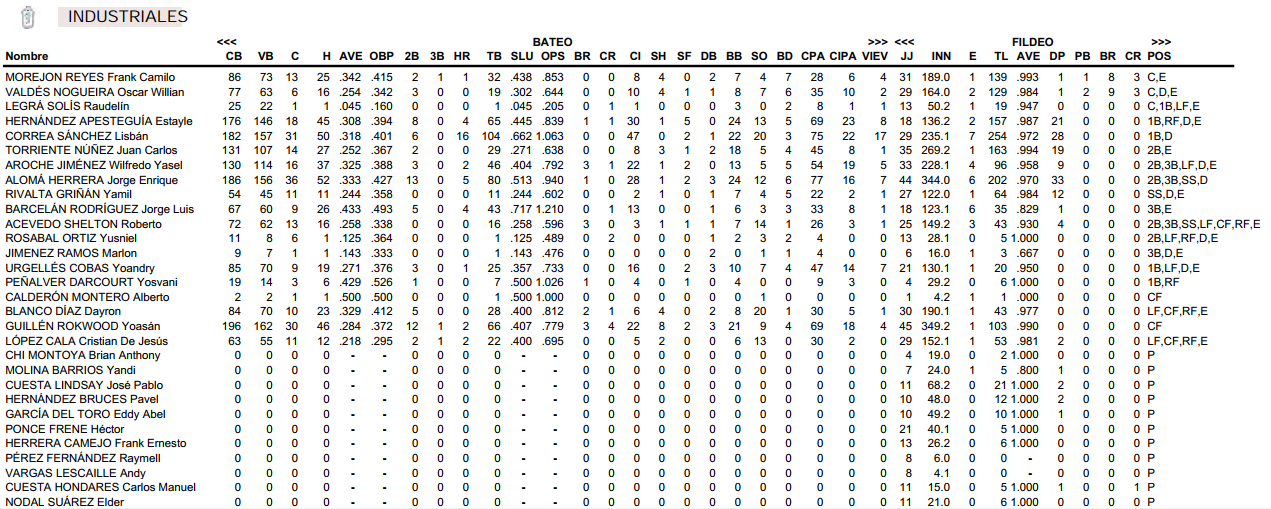
\includegraphics[width=1.3\textwidth]{figuras/informacionPelota.png}
	\caption{Información almacenada de los peloteros en el sitio web beisbolcubano}\label{info-pelota}
\end{figure}

%\end{landscape}
%\end{minipage}
%\vspace{0.5cm}
\newpage
\KOMAoptions{paper=portrait, pagesize}
\recalctypearea

En la Tabla \ref{correspondencia-pel} se presenta la correspondencia entre los indicadores y las competencias técnicas definidas en la sección \ref{compt-pel}. Además de estos indicadores, también existen otros que se pudiesen tener en cuenta, por ejemplo en la \textit{Major Ligue Baseball} (MLB) se maneja la velocidad de \textit{sprint} (SV) expresada en pies/segundos.

\begin{table} [H]
	\centering
	\caption{Correspondencia entre indicadores y competencias técnicas} \label{correspondencia-pel}
	\begin{tabular}{|l|c|}
		\hline
		\textbf{Competencias Técnicas}                                          & \textbf{Indicadores} \\ \hline
		\multirow{4}{5.4cm}{$\boldsymbol{t_1}=batear\;con\;hombres\;en\;base $} &          CI          \\
		                                                                        &          SH          \\
		                                                                        &          SF          \\
		                                                                        &         CIPA/CPA        \\ \hline
		\multirow{4}{5.4cm}{$\boldsymbol{t_2}=fuerza\;de\;bateo $}              &          2B          \\
		                                                                        &          3B          \\
		                                                                        &          HR          \\
		                                                                        &         SLU          \\ \hline
		$\boldsymbol{t_3}= precisi\acute{o}n\;de\;tiro $                        &     AVG (fildeo)     \\ \hline
		\multirow{3}{5.4cm}{$\boldsymbol{t_4}= velocidad $}                     &          BR          \\
		                                                                        &          CR          \\\hline
		$\boldsymbol{t_5}= versatilidad $                                       &         POS          \\ \hline
		\multirow{3}{5.4cm}{$\boldsymbol{t_6}=capacidad\;de\;embase$}           &         OBP          \\
		                                                                        &          BR          \\
		                                                                        &          SH          \\ \hline
	\end{tabular}
\end{table}

En el caso particular de $t_5=velocidad$ se le asocia el indicador \textbf{POS}, este significa la cantidad de posiciones que puede emplear el jugador. A partir de lo planteado en la Tabla \ref{correspondencia-pel} se propone calcular los valores de las competencias técnicas a partir de las siguientes formulaciones:

\begin{flalign}\label{ec:compt}
t_i = \sum_{j=1}^{n_i} c_{ij}*\dfrac{I_j}{R_j} i \neq 4, 5 &&
\end{flalign}

\begin{flalign}
\forall t_{i} \in T \mbox{  se cumple que  } \sum_{j=1}^{n_i} c_{ij} = 1 &&
\end{flalign}

%\vspace{0.5cm}
Donde:
\begin{itemize}
	\item $ c_j $ coeficiente que indica el porcentaje asignado al indicador $I_j$.
	\item $I_j$ indicador que influye en la competencia técnica $t_i$ .
	\item $ R_j $ máximo valor registrado en el equipo para el indicador $ I_j $.
	\item $n_i$ es el número de indicadores que influyen en la competencia técnica $t_i$.
	\item $T$ conjunto de competencias técnicas.
\end{itemize} 

%\vspace{0.5cm}

Todos los coeficientes son configurables y la suma de ellos tiene que ser 1. Para los casos específicos de $ t_4 $ y $t_5$, se proponen utilizar las siguientes fórmulas:

\begin{flalign}\label{ec:embase}
t_4 = \frac{BR}{(BR+CR)} &&
\end{flalign}

\begin{flalign}\label{ec:pos}
t_5 = \frac{C}{9} &&
\end{flalign}

Donde:
\begin{itemize}
	\item $ C $ cantidad de posiciones que juega el jugador. \\
\end{itemize}

Además, el grado de preferencia de los jugadores por los roles se puede obtener a partir de la siguiente formulación:

\begin{flalign}
P_i = \frac{A_i}{E}&&
\end{flalign}

Donde:
\begin{itemize}
	\item $P_i$ preferencia del jugador por el rol $i$.
	\item $A_i$ años de experiencia en el rol $i$.
	\item $E$ años de experiencia como jugador de béisbol.\\
\end{itemize}

Utilizando las formulaciones planteadas, en las Tablas \ref{estadistica-of} y \ref{estadistica-def}  se puede ver un ejemplo de la información necesaria de los peloteros, obtenida del sitio beisbolcubano \cite{INDER2020} para la temporada clasificatoria de la 60 Serie Nacional. En cada una de las tablas anteriores se incluye como última fila, el mayor registro del equipo para cada estadístico. Esta hace referencia al indicador \hyperref[r-sub-j]{$R_j$}, necesario para obtener el valor del jugador en las competencias técnicas. La Tabla \ref{transf-pel} muestra cómo quedaría la normalización a partir de la información de la tablas antes mencionadas. A partir de una revisión de la información histórica manejada en el sitio, se obtuvo los años de experiencia totales de cada jugador. La información utilizada en las Tablas \ref{exp-of}, \ref{exp-def} es ficticia, debido a que no se posee la base de datos, y sin esta, no es posible obtener esa información. Como resultado de la normalización de los años de experiencia jugando cada rol, se construyen las Tablas \ref{pref-rol-of-pel} y \ref{pref-rol-def-pel} , que expresan el grado de preferencia de los jugadores por los roles.

%-------------------------ESTADISTICAS
\begin{table}[H]
	\centering
	\caption{Estadísticas ofensivas de la 60 serie nacional}\label{estadistica-of}
%	\hspace{-2.2cm}
	\begin{tabular}{l c c c c c c c c c }
		\toprule[1.7pt]
		Jugador          & CI & SH & SF & CIPA & 2B & 3B & HR & SLU  & OBP                    \\ \midrule
		Frank Camilo    & 8  & 4  & 0  & 6    & 2  & 1  & 1  & .438 & .415 \\
		Roberto Acevedo & 3  & 1  & 1  & 3    & 0  & 0  & 0  & .258 & .338  \\
		\rowcolor{gray!30} Lisbán Correa   & 47 & 0  & 2  & 22   & 6  & 0  & 16 & .662 & .401  \\ \midrule
		
		\multicolumn{1}{p{4cm}}{Mayor registro equipo} & 47 & 8& 5& 23&15&1&16&.662& .545\\ \bottomrule[1pt]
	\end{tabular}
\end{table}


\begin{table}[H]
		\centering
	\caption{Estadísticas defensivas de la 60 serie nacional}\label{estadistica-def}
%	\hspace{-2.2cm}
		\begin{tabular}{l c c c c}
			\toprule[1.7pt]
			Jugador      &     AVG(fildeo) & BR & CR & POS                    \\ \midrule
			Frank Camilo  &   .993        & 0  & 0  & C                      \\
			Roberto Acevedo&  .930        & 3  & 0  & 2B, 3B, SS, LF, CF, RF \\
			\rowcolor{gray!30} Lisbán Correa   & .972        & 0  & 0  & 1B, BD \\ \midrule
			
			\multicolumn{1}{p{4cm}}{Mayor registro equipo}& 1.000 & 3&4 & 6 posiciones\\ 
			\bottomrule[1pt]
		\end{tabular}
	
\end{table}

A continuación se explica, cómo se pueden calcular los valores de los jugadores para cada competencia técnica utilizando las fórmulas \ref{ec:compt}, \ref{ec:embase}, \ref{ec:pos} y los datos de los jugadores presentados en las Tablas \ref{estadistica-of} y \ref{estadistica-def}. Utilizando al jugador Lisbán Correa (resaltado sus datos en dichas tablas) como ejemplo, se realizan las siguientes operaciones:

\begin{tabular}{l}
	\\
	$t_1 = 0.4 * \dfrac{47}{47} + 0.2 * \dfrac{0}{8} + 0.2 * \dfrac{2}{5} + 0.4 * \dfrac{22}{23} = 0.9$ \\ 
	\\
	$t_2 = 0.1 * \dfrac{6}{15} + 0.2 * \dfrac{0}{1} + 0.35 * \dfrac{16}{16} + 0.35 * \dfrac{662}{662} = 0.68$ \\
	\\
	$t_3 = 1 * \dfrac{972}{1000} = 0.98$ \\
	\\
	$t_4 = \dfrac{0}{0+0} = 0.0$ \\
	\\
	$t_5 = \dfrac{2}{9} = 0.23$ \\
	\\
	$t_6 = 0.7 * \dfrac{401}{545} + 0.15 * \dfrac{0}{8} + 0.15 * \dfrac{0}{8} = 0.58$
\end{tabular}

%\begin{center}
%	\begin{tabular}{lll}
%		$t_1$ = 1.0          &         CP = 1.0    &   T = $\dfrac{2}{10} = 0.2$   \\
%		&&\\
%		S = 1.0          &          L = 1.0     &  JA =$\dfrac{5}{10} = 0.5$  
%	\end{tabular}
%\end{center}

%----------------------------RESULTADOS
\begin{table} [H]
	\centering
	\caption{Resultado de la transformación de las competencias técnicas de los jugadores} \label{transf-pel}
	\begin{tabular}{l | c c >{\columncolor{gray!30}}c }
		\toprule[1.7pt]
		Competencias técnicas                & Frank Camilo & Roberto Acevedo & Lisbán Correa \\ \midrule
		$t_1=batear\;con\;hombres\;en\;base$ & 0.28         & 0.16            & 0.9           \\
		$t_2=fuerza\;de\;bateo$              & 0.55         & 0.12            & 0.68          \\
		$t_3= precisi\acute{o}n\;de\;tiro$   & 1.0          & 0.94            & 0.98          \\
		$t_4=velocidad$                      & 0.0          & 1.0             & 0.0           \\
		$t_5=versatilidad$                   & 0.12         & 0.67            & 0.23          \\
		$t_6=capacidad\;de\;embase$          & 1.0          & 0.59            & 0.58          \\ \bottomrule[1pt]
	\end{tabular}
\end{table}


%------------------------PREFERENCIA


\begin{table}[H]
		\centering
	\caption{Años de experiencia de los jugadores en los roles ofensivos}\label{exp-of}
%	\hspace{-2.2cm}
		\begin{tabular}{l | c c c c c c c c c c}
			\toprule[1.7pt]
			\multicolumn{1}{l}{Personas}   &    \multicolumn{9}{c}{Roles ofensivos}    &  \\ \cline{1-10}
			                                                              & B1 & B2 & B3 & B4 & B5 & B6 & B7 & B8 & B9 &  \\ \cline{2-10}
			Frank Camilo                                                 & 0  & 0  & 0  & 0  & 2  & 6  & 10 & 4  & 16 &  \\
			Roberto Acevedo                                              & 1  & 0  & 0  & 0  & 0  & 1  & 2  & 3  & 5  &  \\
			Lisbán Correa                                                & 0  & 6  & 10 & 8  & 3  & 2  & 0  & 0  & 15 &  \\
			\bottomrule[1pt]                              
		\end{tabular}
	
\end{table}


\begin{table}[H]
	\centering
	\caption{Años de experiencia de los jugadores en los roles defensivos}\label{exp-def}

	\begin{tabular}{l | c c c c c c c c c }
		\toprule[1.7pt]
		\multicolumn{1}{l}{Personas} &    \multicolumn{9}{c}{Roles defensivos}  \\ \cline{1-10}
		                                                           & C  & 1B & 2B & SS & 3B & LF & CF & RF & BD \\ \cline{2-10}
		Frank Camilo                                               & 16 & 0  & 0  & 0  & 0  & 0  & 0  & 0  & 0                           \\
		Roberto Acevedo                                            & 0  & 0  & 2  & 2  & 1  & 4  & 4  & 4  & 0                            \\
		Lisbán Correa                                              & 0  & 12 & 0  & 0  & 0  & 0  & 0  & 0  & 9\\
		\bottomrule[1pt]                             
	\end{tabular}

\end{table}


%----------------------------RESULTADO
\begin{table}[H]
		\centering
	\caption{Preferencia de las personas por los roles ofensivos}\label{pref-rol-of-pel}
%	\hspace{-2.1cm}
	\begin{tabular}{l | c c c c c c c c c}
		\toprule[1.7pt]
		\multicolumn{1}{l}{Personas} &         \multicolumn{9}{c}{Roles ofensivos}         \\ \midrule
		                                                           & B1  & B2  & B3  & B4  & B5  & B6  & B7  & B8  & B9  \\ \cline{2-10}
		Frank Camilo                                               & 0.0 & 0.0 & 0.0 & 0.0 & 0.0 & 0.1 & 0.4 & 0.6 & 0.2 \\
		Roberto Acevedo                                            & 0.2 & 0.2 & 0.0 & 0.0 & 0.0 & 0.0 & 0.2 & 0.4 & 0.6 \\
		Lisbán Correa                                              & 0.0 & 0.0 & 0.4 & 0.6 & 0.5 & 0.2 & 0.1 & 0.0 & 0.0 \\
		\bottomrule[1.2pt]                          
	\end{tabular}
\end{table}

\begin{table}[H]
		\centering
	\caption{Preferencia de las personas por los roles defensivos}\label{pref-rol-def-pel}
		\begin{tabular}{l | c c c c c c c c c }
			\toprule[1.7pt]
			\multicolumn{1}{l}{Personas} &        \multicolumn{9}{c}{Roles defensivos}            \\ \midrule
			& C   & 1B  & 2B  & SS  & 3B  & LF  & CF  & RF  & BD    \\ \cline{2-10}
			Frank Camilo                                               & 1.0 & 0.0 & 0.0 & 0.0 & 0.0 & 0.0 & 0.0 & 0.0 & 0.0  \\
			Roberto Acevedo                                            & 0.0 & 0.0 & 0.4 & 0.4 & 0.2 & 0.8 & 0.8 & 0.8 & 0.0  \\
			Lisbán Correa                                              & 0.0 & 0.8 & 0.0 & 0.0 & 0.0 & 0.0 & 0.0 & 0.0 & 0.6  \\
			\bottomrule[1pt]                              
		\end{tabular}
	
\end{table}
%--------------------------RESULTADOS


\section{Ejemplo simple para el problema de conformación de equipos docentes}

Con el objetivo de adaptar el problema de conformación de equipos docentes al modelo descrito en la sección \ref{sec:modelo-teamsoft}, se muestra mediante un ejemplo, una instancia específica de este problema. A los roles definidos en \ref{ej-carga} se le incorpora el jefe de asignatura (JA), debido a que es un rol importante a tener en cuenta en los equipos docentes. Las asignaturas utilizadas en el ejemplo forman parte del plan de estudio $E$ de la carrera de Ingeniería Informática en la Universidad Tecnológica de La Habana (CUJAE), correspondientes a la disciplina Inteligencia Computacional, estas son: Razonamiento Aproximado (RA) e Inteligencia Artificial (IA).

\subsection{Conjuntos que intervienen en la modelación} \label{conjuntos-docente}
\begin{itemize}
	\item $P=\{p_1, p_2\ldots\}$: Conjunto de personas, $p = 1\ldots |P|$.
	
	\item $T=\{t_1=categor\acute{\i}a\;docente, t_2=grado\;cient\acute{\i}fico, t_3=a\tilde{n}os\;experiencia, t_4=trabajo\;docente, \\t_5=trabajo\;metodol\acute{o}gico, t_6= trabajo\;investigativo\}$: Conjunto de competencias técnicas, $t= 1.. |T|$, $|T|=6$.
	
	\item $G=\{g_1=liderazgo
	, g_2=habilidades\;comunicativas,$ $g_3=pensamiento\;conceptual \footnote{Según \cite{Mayi09} es la habilidad para explicar situaciones o resolver problemas. Desarrollar conceptos nuevos que no resultan obvios para los demás. Hacer que las situaciones o ideas complejas estén claras, sean simples y comprensibles.}, \\ g_4=responsabilidad\}$: Conjunto de competencias genéricas, $g = 1\ldots|G|,\;|G|=4$.
	
	\item $R=\{r_1=C,r_2=CP,r_3=S,r_4=L,r_5=T, r_6=JA\}$: Conjunto de roles, $r,u= 1\ldots|R|$, $|R|=6$.
	
	\item $Y=\{y_1, y_2\}$: Conjunto de asignaturas, $y = 1\ldots |Y|$, $|Y|=2$.
\end{itemize}

En este caso, al igual que en el de béisbol, para una mejor comprensión del problema las relaciones se agrupan en dos secciones: una donde se describen los aspectos generales del proceso docente, y otra específica, donde se tienen en cuenta las características de los profesores con que se cuentan para realizar la planificación de la carga decente. Los valores asignados son todos a consideración del autor y además, son configurables.

\subsection{Elementos generales} \label{asp-gen-doc}

En la Tabla \ref{mcg-carga} se observan los valores necesarios para que una persona pueda jugar un rol según sus competencias genéricas. Por ejemplo, una persona para poder ocupar el rol de profesor de Conferencia (C), es necesario que tenga como valor en la competencia $ g_1  >= 0.5 $. Así sucede con cada competencia asociada a cada rol. 

\begin{table}[H]
	\centering
	\caption{Nivel mínimo requerido de las competencias genéricas para los roles}\label{mcg-carga}
	\begin{tabular}{|l|c|c|c|c|c|c|}
		\hline
		\thead{$Z(g,r)$}                 & $C$ & $CP$ & $S$ & $L$ & $T$ & $JA$ \\ \hline
		$g_1=liderazgo$                  & 0.5 & 0.6  & 0.6 & 0.6 & 0.6 & 0.8  \\ \hline
		$g_2=habilidades\;comunicativas$ & 0.8 & 0.7  & 0.6 & 0.7 & 0.7 & 0.7  \\ \hline
		$g_3=pensamiento\;conceptual$    & 0.8 & 0.8  & 0.7 & 0.7 & 0.7 & 0.8  \\ \hline
		$g_4=responsabilidad$            & 0.8 & 0.8  & 0.7 & 0.7 & 0.7 & 0.8  \\ \hline
	\end{tabular}
\end{table}

En las Tablas \ref{mct1-carga} y \ref{mct2-carga} el valor mínimo que debe tener cada persona en cada una de las competencias requeridas para desempeñar los diferentes roles en la asignatura $y_1$. Como se observa para desempeñar el rol de profesor de conferencia en la asignatura $y_1$, debe tener como mínimo en la competencia técnica $t_2$ 0.8, en cambio para desempeñar ese mismo rol en la asignatura $y_2$ solo debe tener 0.6. Esto se debe a que en dependencia de la asignatura, los valores necesarios en las competencias técnicas
varían.

\begin{table}[H]
	\centering
	\caption{Nivel mínimo requerido de las competencias técnicas para jugar roles en la asignatura $y_1$}\label{mct1-carga}
	\begin{tabular}{|l|c|c|c|c|c|c|}
		\hline
		\thead{$Q(t,r,y_1)$}                & $C$ & $CP$ & $S$ & $L$ & $T$ & $JA$ \\ \hline
		$t_1=categor\acute{\i}a\;docente$   & 0.8 & 0.2  & 0.2 & 0.2 & 0.2 & 0.6  \\ \hline
		$t_2=grado\;cient\acute{\i}fico$    & 0.8 & 0.2  & 0.2 & 0.2 & 0.2 & 0.6  \\ \hline
		$t_3=a\tilde{n}os\;experiencia$     & 0.7 & 0.5  & 0.5 & 0.4 & 0.4 & 0.8  \\ \hline
		$t_4=trabajo\;docente$              & 0.7 & 0.4  & 0.4 & 0.3 & 0.3 & 0.6  \\ \hline
		$t_5=trabajo\;metodol\acute{o}gico$ & 0.6 & 0.4  & 0.4 & 0.4 & 0.4 & 0.8  \\ \hline
		$t_6=trabajo\;investigativo$        & 0.4 & 0.3  & 0.3 & 0.2 & 0.2 & 0.6  \\ \hline
	\end{tabular}
\end{table}

\begin{table}[H]
	\centering
	\caption{Mínimos de las competencias técnicas para jugar roles en la asignatura $y_2$}\label{mct2-carga}
	\begin{tabular}{|l|c|c|c|c|c|c|}
		\hline
		\thead{$Q(t,r,y_2)$}                & $C$ & $CP$ & $S$ & $L$ & $T$ & $JA$ \\ \hline
		$t_1=categor\acute{\i}a\;docente$   & 0.8 & 0.4  & 0.4 & 0.4 & 0.4 & 0.5  \\ \hline
		$t_2=grado\;cient\acute{\i}fico$    & 0.6 & 0.2  & 0.2 & 0.2 & 0.2 & 0.5  \\ \hline
		$t_3=a\tilde{n}os\;experiencia$     & 0.6 & 0.2  & 0.2 & 0.2 & 0.2 & 0.6  \\ \hline
		$t_4=trabajo\;docente$              & 0.6 & 0.3  & 0.3 & 0.2 & 0.2 & 0.5  \\ \hline
		$t_5=trabajo\;metodol\acute{o}gico$ & 0.7 & 0.5  & 0.5 & 0.5 & 0.5 & 0.7  \\ \hline
		$t_6=trabajo\;investigativo$        & 0.5 & 0.4  & 0.4 & 0.3 & 0.3 & 0.6  \\ \hline
	\end{tabular}
\end{table}

%------------nuevo---------------------

Este problema de forma general, no presenta restricciones en cuanto a incompatibilidades entre los roles que puede ejercer un profesor en una asignatura.


\subsection{Elementos específicos}

Cada asignatura tiene sus propias características, al igual que los profesores. En esta sección se ejemplificará el modelo para un conjunto de asignaturas y personas específicos:
\begin{itemize}
	\item $P=\{p_1=lisandra, p_2=wenny, p_3=carlos, p_4=ana\}$: Conjunto de personas, $p, q= 1.. |P|$, $|P|=4$
	
	\item $Y=\{y_1=RA,y_2=IA\}$: Conjunto de asignaturas, $y = 1\ldots |Y|$, $|Y|=2$
\end{itemize}

Del conjunto de roles que puede ejercer un profesor dentro de un colectivo de asignatura, es necesario definir por cada una de ellas, cuáles roles serán planificados (ver Tabla \ref{cpr-carga}) y cuántos profesores se necesitan en cada uno de ellos (ver Tabla \ref{cpnr-carga}). Por ejemplo, en el caso de la asignatura $RA$, se necesitan los roles de conferencia, clase práctica, laboratorio y jefe de asignatura, y se requieren 1, 2, 2 y 1 profesor(es), respectivamente.
\begin{table}[H]
	\centering
	\caption{Roles necesarios por asignatura}\label{cpr-carga}
	\begin{tabular}{|c|c|c|c|c|c|c|}
		\hline
		$K(y,r)$ & $C$ & $CP$& $S$ & $L$ & $T$ & $JA$ \\ \hline
		$y_1=RA$  	 &  1  &  1  &  0  &  1  &  0 &  1\\ \hline
		$y_2=IA$ 	 &  1  &  1  &  1  &  0  &  0 &  1\\ \hline
	\end{tabular}
\end{table}

\begin{table}[H]
	\centering
	\caption{Cantidad de personas necesarias para el rol $r$ en cada asignatura}\label{cpnr-carga}
	\begin{tabular}{|c|c|c|c|c|c|c|}
		\hline
		$K_{p}(r, y)$ & $C$ & $CP$& $S$& $L$& $T$ & $JA$ \\ \hline
		$RA$       &  1  &  2  &  0 &  2 &  0 &  1  \\ \hline
		$IA$       &  2  &  2  &  2 &  0 &  0  & 1 \\ \hline
	\end{tabular}
\end{table}



%\begin{table}[H]
%	\centering
%	\caption{Número de grupos asociados por rol por asignatura}\label{gra-carga}
%	\begin{tabular}{|c|c|c|c|c|c|}
%		\hline
%		$T(r,y)$ & $C$ & $CP$ & $S$ & $L$ & $T$   \\ \hline
%		$RA$  &  2  &   3  &  0  &  3  &  0    \\ \hline
%		$IA$  &  1  &   2  &  2  &  0  &  0    \\ \hline
%	\end{tabular}
%\end{table}

%------------fin nuevo---------------

Este modelo no presenta restricciones en cuanto a la incompatibilidad de los roles. Sin embargo, es posible definir incompatibilidades entre los roles. Esto se establece por el jefe de departamento, que es el encargado de realizar la planificación. Un ejemplo de esto se muestra en las Tablas \ref{ier1-carga} y \ref{ier2-carga}, donde se expresa que el profesor asignado a impartir conferencia no debe estar asignado para impartir clase práctica.

\begin{table}[H]
	\centering
	\caption{Incompatibilidades entre roles en la asignatura $RA$}\label{ier1-carga}
	\begin{tabular}{|c|c|c|c|c|c|c|}
		\hline
		$I_r(r,u,y_1)$  & $C$ & $CP$& $S$ & $L$ & $T$ & $T$  \\ \hline
		$C$  	   		&  0  &  1  &  0  &  0  & 0 & 0	\\ \hline
		$CP$ 	   		&  1  &  0  &  0  &  0  & 0 & 0	\\ \hline
		$S$  	   		&  0  &  0  &  0  &  0  & 0 & 0	\\ \hline
		$L$  	   		&  0  &  0  &  0  &  0  & 0 & 0	\\ \hline
		$T$  	   		&  0  &  0  &  0  &  0  & 0 & 0	\\ \hline
	\end{tabular}
\end{table}

\begin{table}[H]
	\centering
	\caption{Incompatibilidades entre roles en la asignatura $IA$}\label{ier2-carga}
	\begin{tabular}{|c|c|c|c|c|c|c|}
		\hline
		$I_r(r,u,y_2)$  & $C$ & $CP$& $S$ & $L$ & $T$ & $JA$   \\ \hline
		$C$  	   		&  0  &  1  &  1  &  0  & 0 & 0	\\ \hline
		$CP$ 	   		&  1  &  0  &  0  &  0  & 0 & 0	\\ \hline
		$S$  	   		&  1  &  0  &  0  &  0  & 0 & 0	\\ \hline
		$L$  	   		&  0  &  0  &  0  &  0  & 0 & 0	\\ \hline
		$T$  	   		&  0  &  0  &  0  &  0  & 0 & 0	\\ \hline
	\end{tabular}
\end{table}

En dependencia de la asignatura, el tiempo que conlleva desempeñar los roles varía. Por ejemplo en la Tabla \ref{tr-carga} para que un profesor ocupe el rol de Conferencia en la asignatura $RA$, es necesario que tenga libre el 30\% de su tiempo.

\begin{table}[H]
	\centering
	\caption{Tiempo necesario para jugar un rol en una asignatura}\label{tr-carga}
	\begin{tabular}{|c|c|c|c|c|c|c|}
		\hline
		$T(r,y)$ & $C$ & $CP$ & $S$ & $L$ & $T$ & $JA$   \\ \hline
		$RA$    & 0.3 &  0.2 & 0.0 & 0.1 & 0.0  & 0.4  \\ \hline
		$IA$     & 0.4 &  0.3 & 0.1 & 0.0 & 0.0  & 0.4  \\ \hline
	\end{tabular}
\end{table}

Las incompatibilidades entre las personas se ven reflejadas en la Tabla \ref{iep-carga}. Es importante destacar que la relación de incompatibilidad no es la misma en los dos sentidos, por ejemplo, en la Tabla \ref{iep-carga}, $ p_1 $ es medianamente compatible con $ p_2 $, sin embargo, $ p_2 $ es casi incompatible por completo con $ p_1 $.

\begin{table}[H]
	\centering
	\caption{Incompatibilidades entre personas}\label{iep-carga}
	\begin{tabular}{|c|c|c|c|c|}
		\hline
		$I_p(p,q)$ & $p_1$& $p_2$& $p_3$& $p_4$ \\ \hline
		$p_1$  	   & 0.0  &  0.4 & 0.2  &  0.3 \\ \hline
		$p_2$ 	   & 0.9  &  0.0 & 0.9  &  0.0 \\ \hline
		$p_3$      & 0.6  &  0.4 & 0.0  &  0.1 \\ \hline
		$p_4$ 	   & 0.7  &  0.3 & 0.1  &  0.0 \\ \hline
	\end{tabular}
\end{table}

En la Tabla \ref{tp-carga} se observa la carga de tiempo para cada profesor. Por ejemplo $ p_1 $ tiene ocupado el 20\% de su tiempo.

\begin{table}[H]
	\centering
	\caption{Carga de tiempo de las personas}\label{tp-carga}
	\begin{tabular}{|c|c|c|c|c|}
		\cline{2-5}
		\multicolumn{1}{c|}{}& $p_1$ & $p_2$ & $p_3$  & $p_4$ \\ \hline
		$D_d(p)$    & 0.2 & 0.3 & 0.1 & 0.2 \\ \hline
	\end{tabular}
\end{table}

%%------------------------nuevo
%\begin{table}[H]
%	\centering
%	\caption{Carga de tiempo máxima por persona}\label{cmp-carga}
%	\begin{tabular}{|c|c|c|c|c|}
%		\cline{2-5}
%		\multicolumn{1}{c|}{}& $p_1$ & $p_2$ & $p_3$  & $p_4$ \\ \hline
%		$D_m(p)$   &  0.8  &  1.0  &   0.8  &   0.7 \\ \hline
%	\end{tabular}
%\end{table}
%
%%------------------------fin nuevo
La Tabla \ref{pr-carga} refleja el valor de preferencia de las personas por cada rol. Por ejemplo, $p_2$  tiene un nivel muy alto de preferencia sobre el rol  $C$. Mientras que las Tablas \ref{pcg-carga} y \ref{pct-carga} muestran el valor de adecuación de las personas hacia las competencias genéricas y técnicas.

\begin{table}[H]
	\centering
	\caption{Preferencias de las personas por los roles}\label{pr-carga}
	\begin{tabular}{|c|c|c|c|c|c|c|}
		\hline
		$F_r(p,r)$  & $C$ & $CP$ & $S$ & $L$ & $T$  & $JA$ \\ \hline
		$p_1$   	& 0.7 &  0.5 & 0.1 & 0.3 &  0.1 &  0.7 \\ \hline
		$p_2$   	& 1.0 &  0.6 & 0.8 & 0.4 &  0.3 &  0.6  \\ \hline
		$p_3$  	 	& 0.3 &  0.9 & 0.5 & 0.7 &  0.5 &  0.3  \\ \hline
		$p_4$    	& 0.4 &  0.6 & 0.3 & 0.4 &  0.2 &  0.4  \\ \hline
	\end{tabular}
\end{table}

\begin{table}[H]
	\centering
	\caption{Valor de adecuación de las personas a las competencias genéricas}\label{pcg-carga}
	\begin{tabular}{|l|c|c|c|c|}
		\hline
		\thead{$F_g(p,g)$} & $p_1$ & $p_2$ & $p_3$ & $p_4$ \\ \hline
		$g_1=liderazgo$  	   &  1.0  &  0.4  &  0.7 & 0.6 \\ \hline
		$g_2=habilidades\;comunicativas$      &  0.8  &  0.8  &  0.4 & 0.8 \\ \hline
		$g_3=pensamiento\;conceptual$  	   &  1.0  &  0.6  &  0.8 & 0.6 \\ \hline
		$g_4=responsabilidad$  	   &  0.5  &  0.7  &  0.8 & 0.9 \\ \hline
	\end{tabular}
\end{table}

\begin{table}[H]
	\centering
	\caption{Valor de adecuación de las personas a las competencias técnicas}\label{pct-carga}
	\begin{tabular}{|l|c|c|c|c|}
		\hline
		\thead{$F_t(p,t)$} & $p_1$ & $p_2$ & $p_3$ & $p_4$ \\ \hline
		$t_1=categor\acute{\i}a\;docente$  	   &  0.6  &  0.2  &  0.8 &  0.4 \\ \hline
		$t_2=grado\;cient\acute{\i}fico$      &  0.8  &  0.8  &  0.4 &  0.4 \\ \hline
		$t_3=a\tilde{n}os\;experiencia$  	   &  1.0  &  0.4  &  0.4 &  0.6 \\ \hline
		$t_4=trabajo\;docente$     & 0.6 & 0.6 & 0.4 & 0.3 \\ \hline
		$t_5=trabajo\;metodol\acute{o}gico$     & 0.6 & 0.8 & 0.3 & 0.8 \\ \hline
		$t_6=trabajo\;investigativo$     & 0.8 & 0.7 & 0.5 & 0.6 \\ \hline
	\end{tabular}
\end{table}

\subsection{Transformación de los datos}

 En esta sección se propone un método para a partir de los datos almacenados en el sistema de gestión PANDORA identificar cuáles tributan al modelo descrito en la sección anterior. Las Figuras \ref{info-gen-prof} y \ref{horas-prof} son algunas capturas de pantalla del sitio funcionando, y de la información que en él se gestiona. En la Figura \ref{info-gen-prof} se hace referencia a los datos generales de los profesores, como el departamento al que pertenecen, la categoría docente, científica, entre otros. En la Figura \ref{horas-prof} se observa la carga docente acumulada de los profesores, en un año, específicamente en un semestre, expresadas en horas.

\begin{figure} [H]
	\centering
	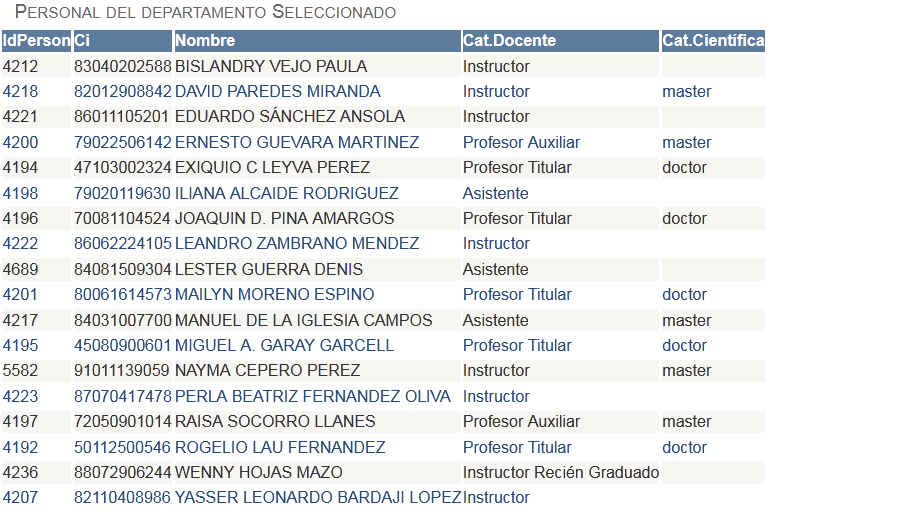
\includegraphics[width=0.9\textwidth]{figuras/catDocCient.png}
	\caption{Información general de los profesores ofrecida por el sistema PANDORA} \label{info-gen-prof}
\end{figure}

\begin{figure} [H]
	\centering
	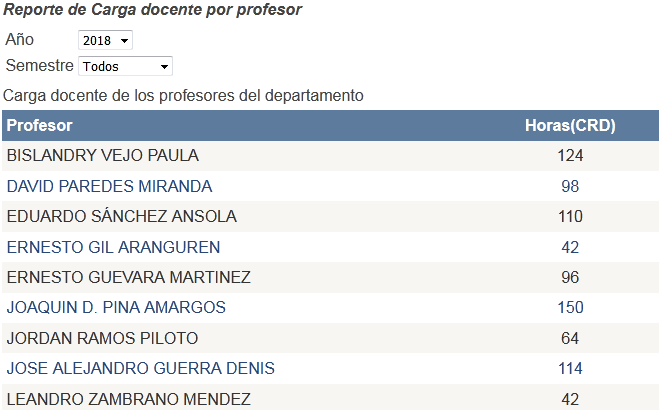
\includegraphics[width=0.7\textwidth]{figuras/HorasProfesor.png}
	\caption{Carga docente} \label{horas-prof}
\end{figure}

Además de los datos mostrados anteriormente, se almacenan los años de experiencia y la evaluación anual del profesor. Esta evaluación incluye seis dimensiones: docente, metodológico, investigación, superación, extensión universitaria y política. En dependencia de las evaluaciones en estas dimensiones se le otorga al profesor una evaluación general a criterio del jefe de departamento. Los resultados de las evaluaciones se expresan en cuatro categorías: Excelente, Bien, Regular, Mal y No Evaluar. \\

En la Tabla \ref{norm-datos-carga} se muestra el proceso de normalización de los datos. Para esto, es necesario otorgar valores numéricos a las categorías docentes, científicas y a las evaluaciones (tanto anual como general). 

\begin{table} [H]
	\centering
	\caption{Normalización de los datos} \label{norm-datos-carga}
	\begin{tabular}{|c|c|c|}
		\cline{2-3}
		             \multicolumn{1}{c|}{}               &    \textbf{Categorías}     & \textbf{Puntuación} \\ \hline
		 \multirow{5}{3cm}{\textbf{Categoría Docente}}   &      Profesor titular      &         1.0         \\ \cline{2-3}
		                                                 &     Profesor Auxiliar      &         0.8         \\ \cline{2-3}
		                                                 &         Asistente          &         0.6         \\ \cline{2-3}
		                                                 &         Instructor         &         0.4         \\ \cline{2-3}
		                                                 & Instructor recién graduado &         0.2         \\ \hline\hline
		\multirow{3}{3cm}{\textbf{Categoría Científica}} &  Doctor en Ciencias(DrC.)  &         1.0         \\ \cline{2-3}
		                                                 & Máster en Ciencias (MsC.)  &         0.5         \\ \cline{2-3}
		                                                 &          Ninguna           &         0.0         \\ \hline\hline
		     \multirow{5}{3cm}{\textbf{Evaluación}}      &         Excelente          &         1.0         \\ \cline{2-3}
		                                                 &            Bien            &         0.8         \\ \cline{2-3}
		                                                 &          Regular           &         0.6         \\ \cline{2-3}
		                                                 &            Mal             &         0.4         \\ \cline{2-3}
		                                                 &       No Evaluación        &         0.0         \\ \hline
	\end{tabular}
\end{table}

Se propone entonces, a partir de lo planteado en la la Tabla \ref{norm-datos-carga}, las siguientes formulaciones para el cálculo de las competencias técnicas establecidas en las sección \ref{conjuntos-docente}:

\begin{flalign}
t_1 = c_d&& \label{ec:cat-doc}\\
t_2 = c_c&&\label{ec:cat-cient}\\
t_3 = \dfrac{A_i}{T}&&\label{ec:exp-prof}\\
t_4 = e_d&&\label{ec:eval-doc}\\
t_5 = e_m&&\label{ec:eval-met}\\
t_6 = e_i&&\label{ec:eval-inv}
\end{flalign}

\vspace{0.3cm}
Donde:
\begin{description}
	\item[(\ref{ec:cat-doc})] $c_d$ corresponde al valor de la categoría docente normalizado.
	\item[(\ref{ec:cat-cient})] $c_c$ corresponde al valor de la categoría  científica normalizado.
	\item[(\ref{ec:exp-prof})] $A_i$ años de experiencia del profesor y $T$ es una constante que sería en máximo número de años de experiencia que puede tener una persona.
	\item[(\ref{ec:eval-doc})] $ e_d $ es el valor normalizado de la evaluación docente.
	\item[(\ref{ec:eval-met})] $ e_m $ es el valor normalizado de la evaluación metodológica.
	\item[(\ref{ec:eval-inv})] $ e_i $ es el valor normalizado de la evaluación investigativa.
\end{description}

%(\ref{ec:cat-cient}) $c_c$ corresponde al valor de la categoría  científica normalizada.\\ \vspace{0.3cm}
%(\ref{ec:exp-prof}) $A$ años de experiencia del profesor y $T$ es una constante que sería en máximo número de años de experiencia que puede tener una persona.\\
%(\ref{ec:eval-doc}) $ e_d $ es el valor normalizado de la evaluación docente.\\
%(\ref{ec:eval-met})$ e_m $ es el valor normalizado de la evaluación metodológica.\\
%(\ref{ec:eval-inv}) $ e_i $ es el valor normalizado de la evaluación investigativa.\\

\vspace{0.3cm}
Además se propone para calcular el grado de preferencia hacia los roles la siguiente fórmula:\\
%$P_i = \displaystyle{\frac{E_i}{A}}$ \\
\begin{flalign}\label{ec:pref-pers}
P_i= \left\{ 
\begin{array}{lcl}
\displaystyle{\frac{E_i}{10}} & \mbox{ si } & E_i < 10 \\
&             &  \\
1.0 & \mbox{ si } & E_i >=10
\end{array}
\right.&&
\end{flalign}

\vspace{0.3cm}
Donde:
\begin{itemize}
	\item $P_i$ el valor de preferencia de la personas por el rol $i$.
	\item $E_i$ años de experiencia del profesor en el rol $i$.
\end{itemize}

\vspace{0.5cm}

Para probar las formulaciones planteadas anteriormente, se utilizarán datos ficticios. En las Tablas \ref{datos-prof1} y  \ref{datos-prof2} se muestra la información necesaria de los profesores. Utilizando el modelo planteado, se obtienen los resultados de la Tabla \ref{result-prof} para las competencias técnicas. La Tabla \ref{exp-prof}  visualiza los años de experiencia de cada profesor impartiendo cada tipo de clases, mientras que la Tabla \ref{trans-prof} refleja la preferencia de los profesores por cada tipo de clases.

\begin{table}[H]
	\centering
	\caption{Datos de los profesores}\label{datos-prof1}
%	\hspace{-2cm}
		\begin{tabular}{l c c c }
			\toprule[1.7pt]
		Profesor(a) & Categoría Docente  & Categoría Científica & Años experiencia \\ \midrule
			Raisa Socorro                             & Profesora Auxiliar & Doctor               & 24               \\
		\rowcolor{gray!30}	Joaquín Pina                              & Profesor Titular   & Doctor               & 25               \\
			Alejandro Rosete                          & Profesor Titular   & Doctor               & 25               \\
			\bottomrule[1pt]            
		\end{tabular}
\end{table}

\begin{table}[H]
	\caption{Evaluación de los profesores}\label{datos-prof2}
	\centering
%	\hspace{-2cm}
	\begin{tabular}{l c c c}
		\toprule[1.7pt]
		Profesor(a) & Trabajo docente & Trabajo metodológico & Trabajo investigativo \\ \midrule
		Raisa Socorro                             & Excelente       & Excelente            & Bien                  \\
		\rowcolor{gray!30} Joaquín Pina                              & Excelente       & Bien                 & Bien                  \\
		Alejandro Rosete                          & Excelente       & Excelente            & Excelente             \\
	\bottomrule[1pt]        
	\end{tabular}
\end{table}




\begin{table}[H]
	\centering
	\caption{Resultado de la transformación de las competencias técnicas de los profesores}\label{result-prof}
%	\hspace{-2cm}
	\begin{tabular}{l c c c}
		\toprule[1.7pt]
		Competencias técnicas & Raisa Socorro & Joaquín Pina & Alejandro Rosete \\ \midrule
		$t_1=categor\acute{\i}a\;docente$                   & 0.8           & 1.0          & 1.0              \\
		$t_2=grado\;cient\acute{\i}fico$                    & 1.0           & 1.0          & 1.0              \\
		$t_4=trabajo\;docente$                              & 1.0           & 1.0          & 1.0              \\
		$t_5=trabajo\;metodol\acute{o}gico$                 & 1.0           & 0.8          & 1.0              \\
		$t_6=trabajo\;investigativo$                        & 0.8           & 0.8          & 1.0              \\
		\bottomrule[1pt]                     
	\end{tabular}
\end{table}

\begin{table}[H]
	\centering
	\caption{Años de experiencia de los profesores}\label{exp-prof}
	\hspace{-2cm}
	\begin{tabular}{l c c c c c c}
		\toprule[1.7pt]
		Profesor(a) & C  & CP & S  & L  & T & JA \\ \midrule
		Raisa Socorro                             & 20 & 10 & 2  & 0  & 2 & 4  \\
		\rowcolor{gray!30} Joaquín Pina                              & 20 & 15 & 12 & 10 & 2 & 5  \\
		Alejandro Rosete                          & 19 & 14 & 7  & 0  & 1 & 10 \\
		\bottomrule[1pt]            
	\end{tabular}
\end{table}

A continuación se explica, cómo se pueden calcular las preferencias de las profesores por los roles utilizando la fórmula \ref{ec:pref-pers} y los datos de los profesores presentados en las Tablas \ref{datos-prof1} y \ref{exp-prof}. Por ejemplo, en el caso del profesor Joaquín Pina (resaltados en gris sus datos en dichas tablas), al tener diez años de experiencia o más en los roles: C, CP, S, y L, el grado de preferencia por cada uno de ellos es el mismo: 1.0. Sin embargo, su experiencia en los roles T y JA es menor de diez años, por lo que al normalizarlos, se obtienen los valores para el grado de preferencia para estos roles de $0.2$ y $0.5$. En la Tabla \ref{trans-prof} se muestran los resultados para todos los profesores cuyos datos están disponibles en las Tablas \ref{datos-prof1} y \ref{exp-prof}.


\begin{table}[H]
	\centering
	\caption{Transformación de los años de experiencia a la preferencia de los profesores por los roles}\label{trans-prof}
	\hspace{-2cm}
	\begin{tabular}{l c c c c c c}
		\toprule[1.7pt]
		Profesor(a) & C   & CP  & S   & L   & T   & JA  \\ \midrule
		Raisa Socorro                             & 1.0 & 1.0 & 0.2 & 0.2 & 0.2 & 0.4 \\
		\rowcolor{gray!30} Joaquín Pina                              & 1.0 & 1.0 & 1.0 & 1.0 & 0.2 & 0.5 \\
		Alejandro Rosete                          & 1.0 & 1.0 & 0.7 & 0.0 & 0.1 & 1.0 \\
		\bottomrule[1pt]          
	\end{tabular}
\end{table}

\section{Limitaciones de la herramienta TEAMSOFT$^+$ para la solución de los problemas de conformación de equipos de béisbol y docentes}

Es necesario comprobar que la herramienta TEAMSOFT$^+$ permite la conformación de los equipos de béisbol y docentes siguiendo las adaptaciones propuestas para ambos problemas. En esta sección se le realizan algunas pruebas a la herramienta para comprobar su funcionamiento ante ambos problemas. \\

Los Casos de Pruebas (CP) se realizaron con las tablas de la base de datos correspondientes a las competencias y roles vacías. Esto persigue como objetivo de simular la creación desde cero de los problemas. Como se observa en la Tabla \ref{t:casos-de-prueba-humo}, en los primeros CP se cumple lo esperado. Mientras que en el CP5, al momento que se intenta crear una nueva estructura, se presenta un error.

\begin{table}[H]
	\centering
	\caption{Prueba de humo crear proyecto sin rol Jefe de Proyecto}\label{t:casos-de-prueba-humo}
	\scalebox{.8}{
		\begin{tabular}{c p{2.3cm} e{4.7cm} p{2cm} p{3cm} p{3cm}}
			\toprule
			\textbf{ID} & \textbf{Escenario} & \item[]\textbf{Pasos} & \textbf{Información de entrada} & \textbf{Resultado esperado} & \textbf{Resultado actual}\\ \midrule
			
			CP1 & Introducir roles sin que el nombre de ninguno sea Jefe de Proyecto & 
			\item Introducir nombre
			\item Introducir descripción
			\item Establecer impacto
			\item Establecer competencias
			\item Establecer incompatibilidades
			& \textit{Primera Base} & El rol debe insertarse sin problemas & Se cumple lo esperado\\ \hline
			
			CP2 & Introducir roles sin que el nombre de ninguno sea Jefe de Proyecto & 
			\item Introducir nombre
			\item Introducir descripción
			\item Establecer impacto
			\item Establecer competencias
			\item Establecer incompatibilidades
			& \textit{Segunda Base} & El rol debe insertarse sin problemas & Se cumple lo esperado\\ \hline
			
			CP3 & Introducir roles sin que el nombre de ninguno sea Jefe de Proyecto & 
			\item Introducir nombre
			\item Introducir descripción
			\item Establecer impacto
			\item Establecer competencias
			\item Establecer incompatibilidades
			& \textit{Capitán} & El rol debe insertarse sin problemas & Se cumple lo esperado\\ \hline
			
			CP4 & Crear Proyecto & 
			\item Abrir menú problema
			\item Introducir nombre
			\item Establecer fecha
			\item Seleccionar entidad
			\item Seleccionar provincia
			& \textit{Nuevo Problema} & Debe continuar con el proceso de creación & Se cumple lo esperado \\ \hline
			
			CP5 & Crear estructura del proyecto & 
			\item Introducir nombre nuevo
			\item Seleccionar roles
			\item Establecer cantidad de trabajadores
			\item \textit{Click} en: Siguiente
			& \textit{Nueva estructura} & Mostrar mensaje creación de la estructura
			 & Se muestra mensaje de error, informando que no hay un jefe de Proyecto entre los roles seleccionados\\ \bottomrule
		\end{tabular}
	}
\end{table}

Los CP que se muestran en la Tabla \ref{t:casos-de-prueba-humo2} se realizaron utilizando los datos que se entraron en los CP1 y CP2 mostrados en la Tabla \ref{t:casos-de-prueba-humo}. En este caso, queda claro que resulta necesario para crear una estructura, que exista un rol con el nombre \textit{Jefe de Proyecto} (ver Figura \ref{fig:error-jefe-proy}).

\begin{table}[H]
	\centering
	\caption{Prueba de humo crear proyecto con rol Jefe de Proyecto}\label{t:casos-de-prueba-humo2}
	\scalebox{.8}{
		\begin{tabular}{c p{2.3cm} e{4.7cm} p{2cm} p{3cm} p{3cm}}
			\toprule
			\textbf{ID} & \textbf{Escenario} & \item[]\textbf{Pasos} & \textbf{Información de entrada} & \textbf{Resultado esperado} & \textbf{Resultado actual}\\ \midrule
			
			CP6 & Introducir rol con nombre Jefe de Proyecto & 
			\item Introducir nombre
			\item Introducir descripción
			\item Establecer impacto
			\item Establecer competencias
			\item Establecer incompatibilidades
			& \textit{Jefe de Proyecto} & El rol debe insertarse sin problemas & Se cumple lo esperado\\ \hline
			
			CP7 & Crear Proyecto & 
			\item Abrir menú problema
			\item Introducir nombre
			\item Establecer fecha
			\item Seleccionar entidad
			\item Seleccionar provincia
			& \textit{Nuevo Problema} & Debe continuar con el proceso de creación & Se cumple lo esperado \\ \hline
			
			CP8 & Crear estructura del proyecto con el rol Jefe de Proyecto incluido & 
			\item Introducir nombre nuevo
			\item Seleccionar roles
			\item Establecer cantidad de trabajadores
			\item \textit{Click} en: Siguiente
			& \textit{Nueva estructura} & La estructura se debe crear correctamente & Se cumple lo esperado\\ \bottomrule
		\end{tabular}
	}
\end{table}

\begin{figure}[H]
	\centering
	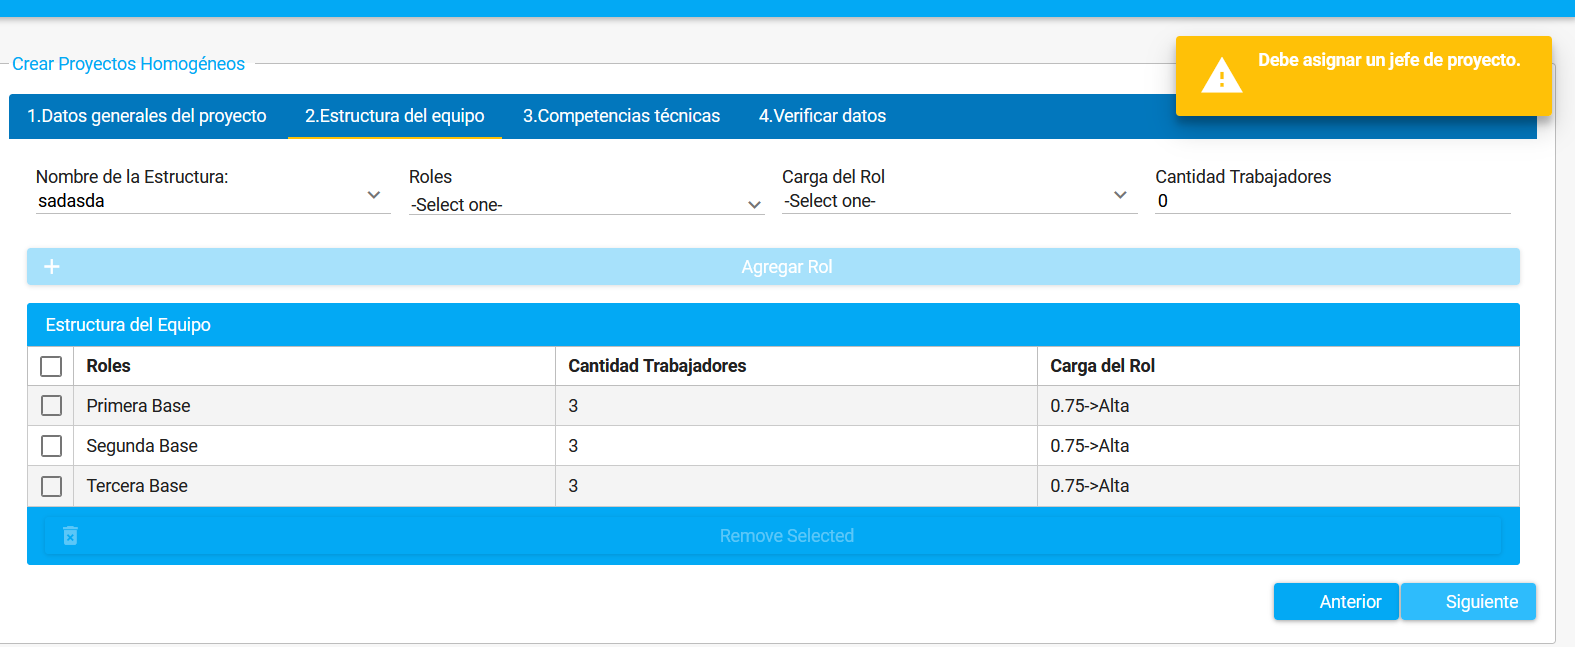
\includegraphics[width=\textwidth]{figuras/error-jefe-proy.png}
	\caption{Error al crear estructura sin Jefe de Proyecto} \label{fig:error-jefe-proy}
\end{figure}

Confirmando lo que muestran los CP realizados, en la Figura \ref{fig:apariciones-jefe-proy} se muestran algunas de las apariciones de la cadena \textit{Jefe de Proyecto} en el código fuente de la herramienta.


\begin{figure}[H]
	\centering
	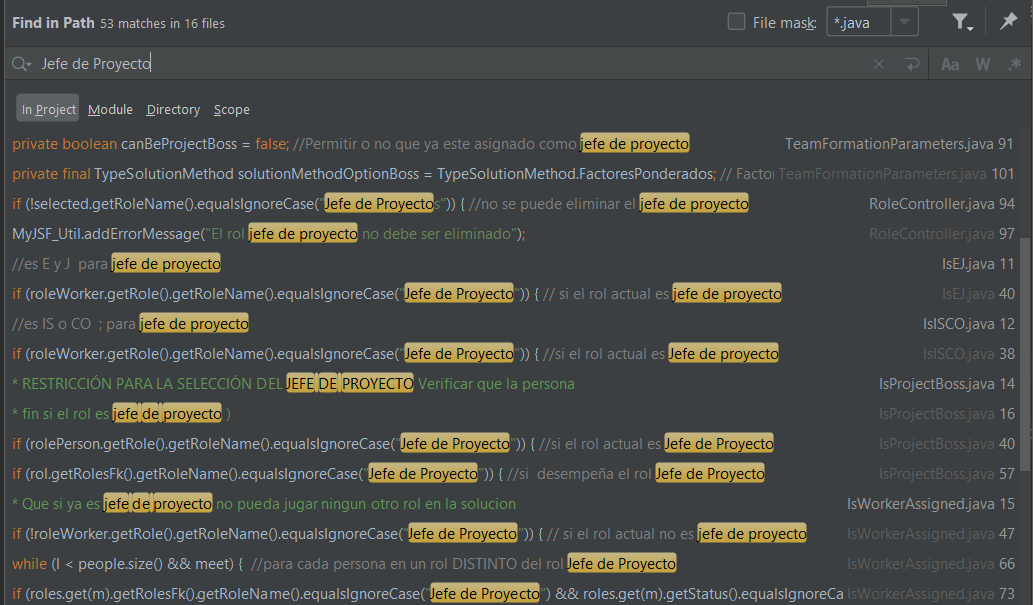
\includegraphics[width=\textwidth]{figuras/string-texto-jefe-proy.png}
	\caption{Apariciones del texto \textit{Jefe de Proyecto}} \label{fig:apariciones-jefe-proy}
\end{figure}

Específicamente para validar que una estructura sea válida, se verifica que en esta exista un rol con el nombre \textit{Jefe de Proyecto}. La Figura \ref{fig:cod-valida} muestra lo planteado.

\begin{figure}[H]
	\centering
	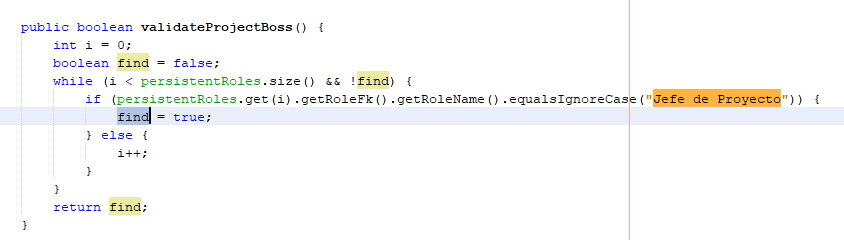
\includegraphics[width=\textwidth]{figuras/validate-state.png}
	\caption{Código utilizado para validar los roles asignados al proyecto} \label{fig:cod-valida}
\end{figure}

%La existencia de una comparación explícita con el nombre del rol no se considera una buena práctica. Lo ideal sería que los roles tengan un campo que se llame líder, y que la validación se realice por este campo. Lo cual llevaría cambios en la base de datos. \\\\


\section{Conclusiones parciales}

Con la culminación de este capítulo, se arribaron a las siguientes conclusiones:
\begin{enumerate}
	\item Es posible aplicar el modelo de conformación de equipos de proyecto para formar equipos docentes y de béisbol. Aunque no se tuvieron en cuenta los roles de Belbin ni los tipos psicológicos de las personas.
	\item La herramienta TEAMSOFT$^+$ presenta algunos problemas para adaptar a los problemas de béisbol y docencia.
	\item Es necesario desarrollar una funcionalidad que permita aplicando fórmulas definidas, importar los datos de las fuentes adecuadas.
\end{enumerate}
